\documentclass[12pt,a4paper]{article}

% ─── Page Layout ───────────────────────────────────────────────────────────────
\usepackage[a4paper, margin=0.8in, headheight=14pt]{geometry}

% ─── Fonts (XeLaTeX) ───────────────────────────────────────────────────────────
\usepackage{fontspec}
\usepackage{unicode-math}
\setmainfont{TeX Gyre Pagella}
\setmonofont[Scale=0.88]{TeX Gyre Cursor}
\setmathfont{Latin Modern Math}

% ─── Packages ──────────────────────────────────────────────────────────────────
\usepackage{xcolor}
\usepackage{colortbl}
\usepackage{titlesec}
\usepackage{enumitem}
\usepackage{tabularx}
\usepackage{booktabs}
\usepackage{array}
\usepackage{amsmath}
\usepackage{tikz}
\usetikzlibrary{shapes.geometric, arrows.meta, positioning, calc, fit, decorations.pathreplacing, patterns}
\usepackage[american]{circuitikz}
\usepackage{tcolorbox}
\tcbuselibrary{skins, breakable}
\usepackage{hyperref}
\usepackage{fancyhdr}
\usepackage{graphicx}
\usepackage{microtype}
\hyphenpenalty=10000
\exhyphenpenalty=10000
\sloppy
\usepackage{caption}
\usepackage{setspace}
\usepackage{multirow}
\usepackage{tocloft}

% ─── Q&A helper ────────────────────────────────────────────────────────────────
\newcommand{\Q}[1]{\textbf{#1}\par\noindent\ignorespaces}

% ─── Colour Palette ────────────────────────────────────────────────────────────
\definecolor{myred}{RGB}{196,30,58}
\definecolor{mydark}{RGB}{30,30,50}
\definecolor{mygreen}{RGB}{14,120,80}
\definecolor{myteal}{RGB}{0,130,140}
\definecolor{myamber}{RGB}{180,100,0}
\definecolor{mypurple}{RGB}{100,30,160}
\definecolor{mygray}{RGB}{246,247,249}
\definecolor{mgframe}{RGB}{180,185,200}
\definecolor{watermark}{RGB}{145,150,170}
\definecolor{hdrred}{RGB}{250,232,235}
\definecolor{hdrgreen}{RGB}{220,244,233}
\definecolor{hdrteal}{RGB}{220,242,244}
\definecolor{hdramber}{RGB}{253,242,215}
\definecolor{hdrpurple}{RGB}{238,228,255}
\definecolor{hdrgray}{RGB}{238,240,245}
\definecolor{rowalt}{RGB}{250,251,253}

% ─── Section Formatting ────────────────────────────────────────────────────────
\titleformat{\section}{\large\bfseries\color{myred}}{\thesection.}{0.5em}{}[\vspace{1pt}{\color{myred}\rule{\linewidth}{0.8pt}}]
\titleformat{\subsection}{\normalsize\bfseries\color{myteal}}{\thesubsection}{0.5em}{}
\titlespacing*{\section}{0pt}{18pt}{7pt}
\titlespacing*{\subsection}{0pt}{11pt}{4pt}

% ─── Paragraph ─────────────────────────────────────────────────────────────────
\setlength{\parindent}{0pt}
\setlength{\parskip}{4pt}

% ─── TOC Styling ───────────────────────────────────────────────────────────────
\renewcommand{\cfttoctitlefont}{\large\bfseries\color{myred}}
\renewcommand{\cftaftertoctitle}{\par\noindent{\color{myred}\rule{\linewidth}{0.8pt}}}
\setlength{\cftbeforetoctitleskip}{0pt}
\setlength{\cftaftertoctitleskip}{6pt}
\renewcommand{\cftsecfont}{\normalsize\bfseries\color{mydark}}
\renewcommand{\cftsecpagefont}{\normalsize\bfseries\color{mydark}}
\renewcommand{\cftsecleader}{\cftdotfill{\cftdotsep}}
\setlength{\cftbeforesecskip}{7pt}
\renewcommand{\cftsubsecfont}{\small\color{mydark}}
\renewcommand{\cftsubsecpagefont}{\small\color{mydark}}
\setlength{\cftbeforesubsecskip}{3pt}
\setlength{\cftsubsecindent}{1.4em}

% ─── Table helpers ─────────────────────────────────────────────────────────────
\renewcommand{\arraystretch}{1.45}
\setlength{\tabcolsep}{6pt}
\arrayrulecolor{mydark}
\newcolumntype{B}[1]{>{\small\bfseries\raggedright\arraybackslash}m{#1}}
\newcolumntype{Y}{>{\small\raggedright\arraybackslash}X}
\renewcommand{\tabularxcolumn}[1]{m{#1}}

% ─── Header / Footer ───────────────────────────────────────────────────────────
\pagestyle{fancy}
\fancyhf{}
\fancyhead[L]{\small\color{myred}\textbf{PE-EC802C}\;\color{mydark}--- VLSI Design Automation}
\fancyhead[R]{\small\color{myteal}\textbf{Module 4 Notes}}
\fancyfoot[C]{\small\color{mydark}\thepage}
\fancyfoot[R]{\small\color{watermark}\textit{\copyright\ Biraj Sarkar}}
\renewcommand{\headrulewidth}{0.5pt}
\renewcommand{\footrulewidth}{0.3pt}

% ─── Hyperref ──────────────────────────────────────────────────────────────────
\hypersetup{colorlinks=true, linkcolor=myteal, urlcolor=myteal,
  pdfauthor={Biraj Sarkar}, pdftitle={PE-EC802C --- Module 4 Notes}}

% ─── tcolorbox styles ──────────────────────────────────────────────────────────
\tcbset{
  tikzbox/.style={colback=mygray, colframe=mgframe, boxrule=0.6pt, arc=4pt,
    left=8pt, right=8pt, top=6pt, bottom=6pt,
    colbacktitle=mgframe, coltitle=mydark, fonttitle=\small\bfseries},
  defbox/.style={colback=hdrgreen, colframe=mygreen, boxrule=0.8pt, arc=4pt,
    left=9pt, right=9pt, top=6pt, bottom=6pt,
    colbacktitle=mygreen, coltitle=white, fonttitle=\small\bfseries},
  formulabox/.style={colback=hdrteal, colframe=myteal, boxrule=0.8pt, arc=4pt,
    left=9pt, right=9pt, top=7pt, bottom=7pt,
    colbacktitle=myteal, coltitle=white, fonttitle=\small\bfseries},
  examplebox/.style={colback=hdramber, colframe=myamber, boxrule=0.8pt, arc=4pt,
    left=9pt, right=9pt, top=6pt, bottom=6pt,
    colbacktitle=myamber, coltitle=white, fonttitle=\small\bfseries},
  masonbox/.style={colback=hdrpurple, colframe=mypurple, boxrule=0.8pt, arc=4pt,
    left=9pt, right=9pt, top=6pt, bottom=6pt,
    colbacktitle=mypurple, coltitle=white, fonttitle=\small\bfseries},
  exambox/.style={colback=hdrpurple, colframe=mypurple, boxrule=1pt, arc=5pt,
    left=10pt, right=10pt, top=8pt, bottom=8pt,
    colbacktitle=mypurple, coltitle=white, fonttitle=\bfseries,
    breakable, title after break={\textbf{Frequently Asked / Viva Questions (contd.)}}}
}
\tcbset{breakable}

% ─── TikZ styles ───────────────────────────────────────────────────────────────
\tikzset{
  block/.style={rectangle, draw=myteal, fill=hdrteal,
    text width=2.4cm, align=center, minimum height=0.95cm,
    font=\small, rounded corners=3pt, line width=0.7pt},
  redblock/.style={rectangle, draw=myred, fill=hdrred,
    text width=2.4cm, align=center, minimum height=0.95cm,
    font=\small, rounded corners=3pt, line width=0.7pt},
  sumjunc/.style={circle, draw=myamber, fill=hdramber,
    minimum size=0.62cm, font=\small, line width=0.8pt},
  arrow/.style={-Stealth, thick, color=mydark},
  line/.style={thick, color=mydark}
}

% ═══════════════════════════════════════════════════════════════════════════════
\begin{document}
% ═══════════════════════════════════════════════════════════════════════════════

\begin{center}
  {\LARGE\bfseries\color{myred} PE-EC802C --- VLSI Design Automation}\\[5pt]
  {\normalsize\color{mydark} Semester VIII \quad$\bullet$\quad 3L:0T:0P \quad$\bullet$\quad 3 Credits}\\[3pt]
  {\normalsize\color{myteal}\textbf{Module 4: VLSI Simulation \& Logic Synthesis}}\\[3pt]
  {\small\color{mydark} CGEC \;$|$\; B.Tech ECE (2023--27) \;$|$\; \textit{Biraj Sarkar}}
\end{center}
\vspace{2pt}
\noindent{\color{myred}\rule{\linewidth}{1.5pt}}
\vspace{2pt}

\hypersetup{linkcolor=mydark}
\tableofcontents
\hypersetup{linkcolor=myteal}
\newpage

% ===============================================================================
\section{VLSI Simulation Techniques}
% ===============================================================================

\begin{tcolorbox}[defbox, title={VLSI Simulation}]
  \textbf{VLSI Simulation} is the process of building a software model of a digital circuit and executing it with test input sequences to verify its functional correctness, check signal timings, and isolate design faults prior to physical fabrication.
\end{tcolorbox}

\subsection{Gate-Level Event-Driven Simulation}
Event-driven simulators calculate logic outputs only when an input signal transition (an \textit{event}) occurs. This is highly efficient because less than $10\%$ of gates in a typical digital circuit switch states during any clock cycle.
\begin{itemize}[leftmargin=*, itemsep=2pt]
  \item \textbf{Event Queue:} Stores pending signal updates sorted by execution time.
  \item \textbf{Time Wheel:} A circular queue scheduling events at future times. A pointer represents current simulation time ($t$). When the pointer moves to slot $i$, the events linked to $t_i$ are evaluated. If a gate output changes, new events are scheduled at $t_i + d$ (where $d$ is gate delay).
\end{itemize}

\begin{tcolorbox}[tikzbox, title={Time Wheel Scheduler Concept}]
\centering
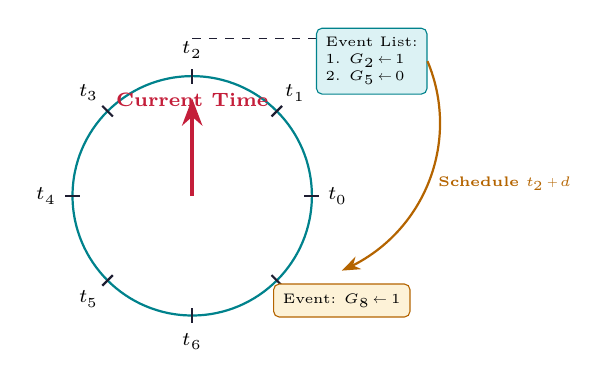
\begin{tikzpicture}[scale=0.95]
  % Draw Time Wheel (circle)
  \draw[line, thick, color=myteal] (0,0) circle (1.6cm);
  \foreach \angle/\time/\label in {0/0/t_0, 45/1/t_1, 90/2/t_2, 135/3/t_3, 180/4/t_4, 225/5/t_5, 270/6/t_6, 315/7/t_7} {
    \draw[line] (\angle:1.5cm) -- (\angle:1.7cm);
    \node[font=\scriptsize\bfseries] at (\angle:1.95cm) {$\label$};
  }

  % Pointer
  \draw[arrow, line width=1.5pt, color=myred] (0,0) -- (90:1.3cm) node[above, pos=0.8, font=\scriptsize\bfseries] {Current Time};

  % Event list hanging from t_2 (90 deg)
  \draw[dashed, color=mydark] (90:2.1cm) -- ++(1.8,0);
  \node[draw=myteal, fill=hdrteal, rounded corners=2pt, font=\tiny, align=left] (list) at (2.4, 1.8) {Event List:\\1. $G_2 \leftarrow 1$\\2. $G_5 \leftarrow 0$};

  % Future event scheduling arrow
  \draw[arrow, bend left=45, color=myamber] (list.east) to node[midway, right, font=\tiny\bfseries] {Schedule $t_2 + d$} (2.0,-1.0);
  \node[draw=myamber, fill=hdramber, rounded corners=2pt, font=\tiny] at (2.0,-1.4) {Event: $G_8 \leftarrow 1$};
\end{tikzpicture}
\end{tcolorbox}

\subsection{Switch-Level Simulation}
Models digital circuits at the transistor level by representing MOS transistors as voltage-controlled switches.
\begin{itemize}[leftmargin=*, itemsep=2pt]
  \item \textbf{States:} Signals are modeled using more than two states, usually including $0$ (low), $1$ (high), $X$ (unknown), and $Z$ (high impedance).
  \item \textbf{Strengths:} Signals are assigned strengths to resolve bus contention (e.g. supply strength, pull strength, charge storage strength). An active pull-up transistor overrides a weak pull-down resistor.
\end{itemize}

\subsection{Compiled-Code vs. Event-Driven Simulation}
Gate-level simulators evaluate logic gates using two primary simulation paradigms:
\begin{itemize}[leftmargin=*, itemsep=3pt]
  \item \textbf{Compiled-Code Simulation:} The digital circuit is translated into a sequence of machine instructions that are executed line-by-line. It evaluates the logic value of every gate in strict topological order during every simulation cycle, regardless of whether its input values have changed. It is highly efficient for circuits with very high switching activity, but extremely wasteful for typical circuits where only a small fraction ($<10\%$) of gate inputs change state at any step.
  \item \textbf{Event-Driven Simulation:} Only evaluates a logic gate when a transition (event) occurs on at least one of its inputs. It schedules events dynamically using a priority queue (event queue or time wheel). While it avoids redundant gate evaluations, it incurs runtime overhead for queue management. It is the preferred method for large digital systems with low-to-medium active switching.
\end{itemize}

\par\vspace{6pt}\noindent
{\renewcommand{\arraystretch}{1.35}%
\begin{tabularx}{\linewidth}{|B{3.2cm}|Y|Y|}
\hline
\textbf{Feature} & \textbf{Compiled-Code Simulation} & \textbf{Event-Driven Simulation} \\
\hline
Evaluation Rule & Evaluates all gates in every simulation cycle. & Evaluates gates only when input signals switch states. \\
\hline
Overhead & Zero scheduling or queue management overhead. & Dynamic scheduling and queue sorting overhead. \\
\hline
Optimal Activity & Best suited for high switching activity circuits. & Best suited for low-to-medium switching activity ($<10\%$). \\
\hline
Delay Modeling & Strictly cycle-based; difficult to model gate delays. & Models detailed gate propagation and inertial delays. \\
\hline
\end{tabularx}}

% ===============================================================================
\section{Combinational Logic Synthesis}
% ===============================================================================

Logic synthesis converts high-level RTL descriptions (Verilog/VHDL) into an optimized gate-level netlist. The combinational logic synthesis process consists of two primary sequential phases:

\subsection{1. Technology-Independent Optimization}
Optimizes the Boolean behavior of the network without considering specific library gates. The circuit is modeled as a \textbf{Boolean Network} (a Directed Acyclic Graph where nodes represent Boolean functions and edges represent signal flow).
\begin{itemize}[leftmargin=*, itemsep=3pt]
  \item \textbf{Restructuring Operations:}
        \begin{itemize}[leftmargin=*, label=$\bullet$, itemsep=1.5pt]
          \item \textbf{Decomposition:} Splitting a complex node function into smaller, simpler functions.
          \item \textbf{Extraction:} Identifying common sub-expressions across multiple nodes and creating a new node to share them, reducing overall literal count.
          \item \textbf{Factoring:} Converting SOP forms to factored forms (e.g. $ab + ac \rightarrow a(b+c)$) to minimize transistor count.
          \item \textbf{Substitution:} Expressing a node's function in terms of other existing nodes.
          \item \textbf{Collapsing:} Merging a node into its fan-out nodes to eliminate intermediate nodes, reducing delay at the expense of area.
        \end{itemize}
  \item \textbf{And-Inverter Graphs (AIGs):} A representation where every node is a 2-input AND gate, and edges can contain inversion flags. Highly efficient for Boolean reasoning and logic optimization.
\end{itemize}

\subsection{2. Technology Mapping}
Translates the optimized technology-independent Boolean network into standard library cells of the target fabrication process (e.g. static CMOS NAND, NOR, AOI gates).
\begin{itemize}[leftmargin=*, itemsep=3pt]
  \item \textbf{Tree Matching (Dagon's Algorithm):}
        \begin{itemize}[leftmargin=*, label=$\bullet$, itemsep=1.5pt]
          \item The Boolean network is partitioned into a collection of trees.
          \item Library gates are also represented as patterns of trees.
          \item Dynamic programming is applied to find the minimum-cost cover of standard cells that matches the network tree structures.
        \end{itemize}
  \item \textbf{Objectives:} Optimizing for minimum area, minimum delay (critical path), or minimum power dissipation.
\end{itemize}

\section{Two-Level Logic Synthesis}
% ===============================================================================

Logic synthesis compiles high-level RTL descriptions (Verilog/VHDL) into an optimized gate-level netlist. Two-level logic synthesis targets sum-of-products (SOP) forms.

\subsection{Quine-McCluskey (QM) Minimisation}
An exact tabular method that guarantees finding the absolute minimum SOP expression.
\begin{enumerate}[leftmargin=*, itemsep=2.5pt]
  \item Represent minterms in binary and group them by the number of 1s they contain.
  \item Combine minterms that differ by exactly one bit (e.g., $0100$ and $0101$ combine to $010-$), replacing the differing bit with a dash.
  \item Repeat combinations until no more terms can be merged. The remaining uncombined terms are \textbf{Prime Implicants (PI)}.
  \item Construct a Prime Implicant chart, identify \textbf{Essential Prime Implicants (EPI)} (columns containing only one checkmark), and select the minimum subset of PIs to cover the remaining minterms.
\end{enumerate}

\subsection{Espresso Heuristic Minimiser}
Because QM suffers from exponential time complexity ($O(2^{2^n})$) and is unusable for more than 10 inputs, industrial synthesis tools use the Espresso heuristic optimizer.
Key iterative steps in Espresso:
\begin{itemize}[leftmargin=*, itemsep=2pt]
  \item \textbf{Expand:} Squeezes out variables by expanding cubes to cover adjacent minterms, reducing the total number of terms.
  \item \textbf{Irredundant:} Selects a minimum subset of prime cubes that covers the entire ON-set, deleting redundant terms.
  \item \textbf{Reduce:} Shrinks cubes to their smallest possible dimensions without uncovering any minterms, allowing the algorithm to search in new directions during the next Expand phase.
\end{itemize}

% ===============================================================================
\section{Binary Decision Diagrams (BDD)}
% ===============================================================================

\begin{tcolorbox}[defbox, title={Binary Decision Diagram}]
  A \textbf{Binary Decision Diagram (BDD)} is a directed acyclic graph (DAG) representation of a Boolean function. It is constructed by recursively applying Shannon's expansion theorem.
\end{tcolorbox}

\subsection{Shannon's Expansion Theorem}
Any Boolean function $f(x_1, x_2, \dots, x_n)$ can be expanded about variable $x_1$ as:
\begin{equation}
  f = x_1 \cdot f_{x_1} + x_1' \cdot f_{x_1'}
\end{equation}
where $f_{x_1} = f(1, x_2, \dots, x_n)$ is the positive cofactor, and $f_{x_1'} = f(0, x_2, \dots, x_n)$ is the negative cofactor.

\begin{tcolorbox}[examplebox, title={Shannon's Expansion Example}]
\Q{Problem:} Expand the function $f = AB + B'C$ about variable $A$.

\textbf{Solution:}\par\noindent
\begin{enumerate}[leftmargin=*, itemsep=2pt]
  \item Compute cofactors about $A$:
        \begin{align*}
          f_A &= (1)B + B'C = B + C \quad (\text{using absorption } B+B'C = B+C) \\
          f_{A'} &= (0)B + B'C = B'C
        \end{align*}
  \item Combine terms using Shannon's theorem:
        \begin{equation*}
          f = A \cdot (B + C) + A' \cdot (B'C)
        \end{equation*}
\end{enumerate}
\end{tcolorbox}

\subsection{Reduced Ordered BDDs (ROBDD)}
An \textbf{Ordered BDD (OBDD)} is a BDD where variables are evaluated in a fixed order along every path from root to leaf. A \textbf{Reduced OBDD (ROBDD)} is obtained by applying three reduction rules:
\begin{enumerate}[leftmargin=*, itemsep=2pt]
  \item \textbf{Merge Duplicate Leaves:} Combine all leaf nodes containing $0$ into a single $0$-terminal, and all $1$-leaves into a single $1$-terminal.
  \item \textbf{Merge Duplicate Nodes:} If two internal nodes $u$ and $v$ represent the same variable and have identical low and high child nodes, merge them.
  \item \textbf{Eliminate Redundant Nodes:} If an internal node has the same low and high child node $w$, delete the node and redirect all incoming edges directly to $w$.
\end{enumerate}

\begin{tcolorbox}[tikzbox, title={BDD to ROBDD Reduction Steps}]
\centering
\begin{minipage}{0.48\linewidth}
\centering
\textbf{Unreduced BDD:}\par\noindent
\vspace{6pt}
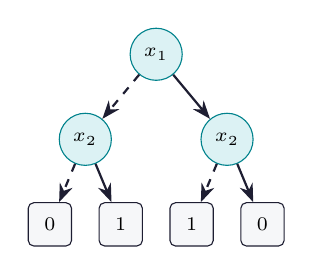
\begin{tikzpicture}[scale=0.9, every node/.style={circle, draw=myteal, fill=hdrteal, minimum size=0.55cm, font=\scriptsize}]
  \node (x1) at (1.5,2.4) {$x_1$};
  \node (x2a) at (0.5,1.2) {$x_2$};
  \node (x2b) at (2.5,1.2) {$x_2$};
  
  \node[rectangle, rounded corners=2pt, draw=mydark, fill=mygray] (z0a) at (0,0) {0};
  \node[rectangle, rounded corners=2pt, draw=mydark, fill=mygray] (z1a) at (1.0,0) {1};
  \node[rectangle, rounded corners=2pt, draw=mydark, fill=mygray] (z1b) at (2.0,0) {1};
  \node[rectangle, rounded corners=2pt, draw=mydark, fill=mygray] (z0b) at (3.0,0) {0};

  % Edges (solid = high/1, dashed = low/0)
  \draw[arrow, dashed] (x1) -- (x2a);
  \draw[arrow] (x1) -- (x2b);
  
  \draw[arrow, dashed] (x2a) -- (z0a);
  \draw[arrow] (x2a) -- (z1a);
  
  \draw[arrow, dashed] (x2b) -- (z1b);
  \draw[arrow] (x2b) -- (z0b);
\end{tikzpicture}
\end{minipage}\hfill
\begin{minipage}{0.48\linewidth}
\centering
\textbf{Reduced ROBDD (after merging):}\par\noindent
\vspace{6pt}
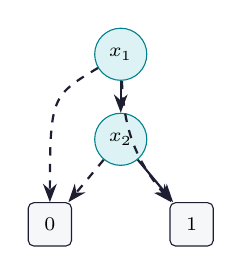
\begin{tikzpicture}[scale=0.9, every node/.style={circle, draw=myteal, fill=hdrteal, minimum size=0.55cm, font=\scriptsize}]
  \node (x1) at (1.5,2.4) {$x_1$};
  \node (x2) at (1.5,1.2) {$x_2$};
  
  \node[rectangle, rounded corners=2pt, draw=mydark, fill=mygray] (z0) at (0.5,0) {0};
  \node[rectangle, rounded corners=2pt, draw=mydark, fill=mygray] (z1) at (2.5,0) {1};

  % Edges
  \draw[arrow, dashed] (x1) .. controls (0.5,1.8) .. (z0);
  \draw[arrow] (x1) -- (x2);
  
  \draw[arrow, dashed] (x2) -- (z0);
  \draw[arrow] (x2) -- (z1);
  
  \draw[arrow, dashed, bend right=20] (x1) to (z1);
\end{tikzpicture}
\end{minipage}
\tcblower
ROBDDs are canonical representations of Boolean functions. For a fixed variable ordering, every Boolean function has exactly one unique ROBDD.
\end{tcolorbox}

\subsection{The BDD Apply Operation}
The BDD \textbf{Apply} algorithm is the fundamental operation used to combine two BDDs with a binary Boolean operator (such as AND, OR, XOR). Given BDDs for $f$ and $g$, the algorithm computes the BDD for $h = f \text{ op } g$ in $O(|f| \cdot |g|)$ polynomial time.

\textbf{Recursive Algorithm Principle (Shannon Expansion):}
Let $x$ be the variable with the highest priority (lowest index in the variable ordering) among the root variables of BDDs $f$ and $g$. We can expand $f \text{ op } g$ about $x$ as:
\begin{equation}
  f \text{ op } g = x \cdot (f_x \text{ op } g_x) + x' \cdot (f_{x'} \text{ op } g_{x'})
\end{equation}
where $f_x$ and $f_{x'}$ are cofactors of $f$ with respect to $x$ ($f_x = f(1)$ and $f_{x'} = f(0)$). If $f$ does not depend on $x$, then $f_x = f_{x'} = f$.

\textbf{Algorithmic Flow:}
\begin{enumerate}[leftmargin=*, itemsep=2pt]
  \item \textbf{Base Cases:} If $f$ and $g$ are terminal nodes ($0$ or $1$), evaluate the operation directly (e.g., $1 \text{ AND } 0 = 0$).
  \item \textbf{Memoization (Computed Table):} Before recursively expanding, check if the triple $(f, g, \text{op})$ has already been computed. If yes, return the cached result. This avoids exponential recursive redundancy.
  \item \textbf{Recursion:} Compute the cofactors, and recursively call the Apply algorithm on the positive cofactors $h_{\text{high}} = \text{Apply}(\text{op}, f_x, g_x)$ and negative cofactors $h_{\text{low}} = \text{Apply}(\text{op}, f_{x'}, g_{x'})$.
  \item \textbf{Reduction:} If $h_{\text{high}} == h_{\text{low}}$, return $h_{\text{low}}$ (redundant node elimination). Otherwise, find or create a node for variable $x$ pointing to $h_{\text{high}}$ (as high child) and $h_{\text{low}}$ (as low child), and store the result in the computed table.
\end{enumerate}

\newpage

% ═══════════════════════════════════════════════════════════════════════════════
% QUICK REVISION PAGE
% ═══════════════════════════════════════════════════════════════════════════════
\begin{center}
  {\large\bfseries\color{myred} Quick Revision — Module 4}\\[3pt]
  {\small\color{mydark} Logic Synthesis, Simulation \& BDDs $|$ PE-EC802C}
\end{center}
\noindent{\color{myred}\rule{\linewidth}{1.2pt}}
\vspace{8pt}

\begin{tcolorbox}[formulabox, title={\textbf{Key Formulas and Metrics at a Glance}}]
\renewcommand{\arraystretch}{1.35}
\begin{tabularx}{\linewidth}{B{5.0cm} X}
  Shannon's Expansion & $f = x_i \cdot f_{x_i} + x_i' \cdot f_{x_i'} \quad (\text{foundation for BDD node building})$ \\[4pt]
  QM Worst-Case Implicants & $N_{\text{PI}} \approx \dfrac{3^n}{n} \quad (\text{for } n \text{ variables})$ \\[4pt]
  Event Scheduler Delay & $t_{\text{schedule}} = t_{\text{current}} + d_{\text{gate}} \quad (\text{event propagation delay})$
\end{tabularx}
\end{tcolorbox}

\vspace{6pt}

\begin{tcolorbox}[defbox, title={\textbf{One-Line Definitions}}]
\begin{itemize}[leftmargin=*, itemsep=3pt, topsep=0pt]
  \item \textbf{Time Wheel:} A circular scheduler queue used in event-driven simulators to track gate updates.
  \item \textbf{Switch-Level:} Transistor-level logic simulation where nodes represent strengths and states.
  \item \textbf{Prime Implicant:} A product term (cube) that cannot be combined with any other term to form a simpler term.
  \item \textbf{EPI:} A prime implicant that covers at least one minterm not covered by any other prime implicant.
  \item \textbf{Espresso:} An industrial heuristic logic minimizer that runs in polynomial average time.
  \item \textbf{Cofactor:} The Boolean function obtained by setting a specific variable to 0 or 1.
  \item \textbf{ROBDD:} A canonical directed acyclic graph representing a Boolean function, minimized using reduction rules.
  \item \textbf{Canonical Form:} A unique representation of a mathematical object, allowing easy comparison.
\end{itemize}
\end{tcolorbox}

\vspace{6pt}

\begin{tcolorbox}[exambox, title={\textbf{Frequently Asked / Viva Questions}}]
\begin{enumerate}[leftmargin=*, topsep=0pt, label=\textbf{Q\arabic*.}, itemsep=6pt]
  \item \Q{Explain the advantage of event-driven simulation over compiler-driven simulation.}
        Compiler-driven simulation evaluates every gate in the circuit during every time step, which is slow. Event-driven simulation only evaluates gates whose inputs undergo a transition (an event). Since only $2-10\%$ of gates change states in a clock cycle, event-driven simulation is 10 times faster.
        
  \item \Q{Why are multiple strengths used in switch-level simulators?}
        Transistors can have different dimensions, driving strengths, or functions (e.g. pull-up vs. pull-down). Using strengths allows the simulator to resolve contentions when multiple transistors drive the same bus line, ensuring that the stronger driver dominates.
        
  \item \Q{What is the difference between Quine-McCluskey (QM) and Espresso?}
        QM is an exact minimization algorithm that guarantees the absolute minimum SOP form but has exponential time complexity. Espresso is a heuristic optimizer that uses Expand, Reduce, and Irredundant steps to find a near-optimal solution in polynomial average time, making it suitable for large circuits.
        
  \item \Q{Why is variable ordering critical in ROBDDs?}
        The size (number of nodes) of an ROBDD is highly sensitive to the chosen variable order. A good ordering can result in a linear number of nodes ($O(n)$), while a poor ordering can make the node count grow exponentially ($O(2^n)$) for the exact same function.
        
  \item \Q{What are cofactors, and how are they used in logic synthesis?}
        A cofactor is a simplified Boolean function obtained by setting a variable to a constant value ($f_{x_i} = f(x_i = 1)$). They are used in Shannon's expansion to recursively build BDDs and simplify logic expressions.
        
  \item \Q{How does the Espresso algorithm use the "Reduce" operation to escape local minima?}
        The Reduce operation shrinks the size of prime cubes. This temporarily exposes some minterms, allowing the subsequent Expand step to expand cubes in different directions. This cycle helps the algorithm escape local minima.
        
  \item \Q{What is a canonical representation, and why are ROBDDs canonical?}
        A canonical representation is a unique way of writing a mathematical object. ROBDDs are canonical because, for a fixed variable ordering, any Boolean function has exactly one unique ROBDD structure. This allows checking if two functions are identical in $O(1)$ constant time.
        
  \item \Q{Explain the "Merge Duplicate Leaves" reduction rule in BDDs.}
        This rule combines all leaf nodes containing $0$ into a single $0$-terminal, and all leaves containing $1$ into a single $1$-terminal. This reduces the node count and creates a single converging point for all paths.
        
  \item \Q{What is the function of the event queue in an event-driven simulator?}
        The event queue stores pending signal changes sorted by their execution times. As the simulator moves forward, it fetches events from the current time slot, evaluates the affected gates, and schedules new events at future slots.
        
  \item \Q{Why do we need logic synthesis tools?}
        Logic synthesis automatically translates high-level functional code (Verilog/VHDL) into an optimized gate netlist. This speeds up design, guarantees logical correctness, and optimizes the gate count to meet timing and area constraints.
\end{enumerate}
\end{tcolorbox}

\vspace{6pt}

\begin{tcolorbox}[tikzbox, title={\textbf{Comparison Snapshot}}]
\textbf{Gate-Level vs. Switch-Level Simulation:}\par\vspace{6pt}\noindent
{\renewcommand{\arraystretch}{1.35}%
\begin{tabularx}{\linewidth}{|B{3.2cm}|Y|Y|}
\hline
\textbf{Feature} & \textbf{Gate-Level Simulator} & \textbf{Switch-Level Simulator} \\
\hline
Primitive Element & Boolean logic gates (AND, OR, XOR). & MOS transistors (nodes, switches). \\
\hline
Execution Speed & Very fast (evaluates only on logic changes). & Slow (calculates charge flows and transistor strengths). \\
\hline
Accuracy & Ideal logic behavior. & Captures bi-directional pass transistor behavior. \\
\hline
\end{tabularx}}

\vspace{12pt}
\textbf{BDD vs. ROBDD:}\par\vspace{6pt}\noindent
{\renewcommand{\arraystretch}{1.35}%
\begin{tabularx}{\linewidth}{|B{3.2cm}|Y|Y|}
\hline
\textbf{Feature} & \textbf{Binary Decision Diagram (BDD)} & \textbf{Reduced Ordered BDD (ROBDD)} \\
\hline
Ordering & No fixed order of variables along paths. & Strict, identical variable ordering along all paths. \\
\hline
Uniqueness & Not unique (multiple representations). & Canonical (unique representation). \\
\hline
Leaf Nodes & Contains duplicate $0$ and $1$ terminal leaves. & Contains exactly one $0$ and one $1$ terminal. \\
\hline
\end{tabularx}}
\end{tcolorbox}

\end{document}
